\newpage
\hypertarget{sec:breakpoints}{}
\section{Integrator Breakpoints}
\genHeader

Now that we have two rules to handle partitions, there'S the potential for things to go wrong. Suppose you're debugging, and want to know when in the
transformation, you start to handle any extra partitions, outside of the three permitted in \texttt{BoxToDictionaryRule}. As we saw in the previous sections, it
can sometimes take a long time to run through the integrator step by step, especially so if you have a solid number of rules.  Lets finally discuss the
\texttt{BreakPointSet.xmi} file that's created when you run the integrator for the first time.

\begin{itemize}

\item[$\blacktriangleright$] Double-click the file to open it, and create a new \texttt{Rule Name} break point (Fig.~\ref{eclipse:breakpointChild}).

\begin{figure}[htbp]
\begin{center}
  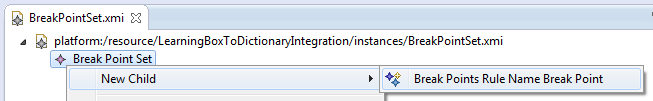
\includegraphics[width=\textwidth]{eclipse_breakpointChild}
  \caption{stuff}
  \label{eclipse:breakpointChild}
\end{center}
\end{figure}

\item[$\blacktriangleright$] Edit its \texttt{Rule Name} property below the editor to \texttt{AllOtherCardsRule} (Fig.~\ref{eclipse:bpProps}). This will create
a breakpoint and stop the integrator/transformation when it's about to apply the rule. Save the file.

\begin{figure}[htbp]
\begin{center}
  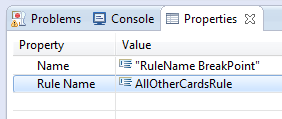
\includegraphics[width=0.5\textwidth]{eclipse_breakpointProperties}
  \caption{stuff}
  \label{eclipse:bpProps}
\end{center}
\end{figure}

\item[$\blacktriangleright$] Run the integrator on \texttt{corr\_FWD} and drag in the breakpoint model before \texttt{protocol\_FWD}. A small note will appear
stating that it is setting the breakpoints.

\item[$\blacktriangleright$] Drag in \texttt{protocol\_FWD}. You are now able to quickly run forwards through the transformation by pressing
\texttt{alt+shift+ctrl+RIGHT} or backwards with \texttt{alt+shift+ctrl+LEFT}. This may be useful for both debugging or testing. 

\item[$\blacktriangleright$] Note that this breakpoint doesn't stop the integrator when used on the backward correspondence. This is because
\texttt{AllOtherCardsRule} only operates in the source domain, and is never called in the reverse direction. If you edit the rule name to
\texttt{BoxToDictionaryRule}, it will work in both directions, as that rules edits the file in both directions.

\end{itemize}
